\chapter*{Questão 1}

\section*{Enunciado}
\noindent 1. A fim de testarmos o gerador de números aleatórios calculemos alguns momentos da 
distribuição ``aleatória'' gerada, isto é:

\begin{equation}
  \langle x^n \rangle, \quad \text{para } n = 1,2,3,4.
\end{equation}

\noindent Faça a média acima gerando um número grande $N$ de números aleatórios (escolha 
apropriadamente $N$). Que resultado você esperaria? Compare com os resultados esperados 
e explique os obtidos.

\section*{Método utilizado}
Na primeira simulação, foi pedido para encontrar a média da distribuição de números aleatórios, 
que variam de 0 a 1 os quais estão sendo elevados por uma potência n, Equação \ref{equation_1}. 
Desse modo, foi utilizado a função \textbf{rand()}, para gerar números aleatórios entre 0 e 1, ademais, 
foi dado uma \textit{seed} para ela, o que permite a função gerar números pseudo randômicos baseados no valor dado.

\begin{equation} \label{equation_1}
    \langle x^n \rangle, \quad \text{para } n = 1,2,3,4.
\end{equation}

Além disso, foram dadas $10^6$ interações, ou seja, foram gerados $10^6$ números pseudo-aleatórios. 
Dessa forma, primeiro foi feito um \textit{loop} na qual o exponencial dos números aleatórios, \textit{n}, varia de 1 a 4, 
e para cada expoente é chamado uma função que realiza o cálcula da média dos valores aleatórios elevados n. 
Por fim, o resultado final é divido pelo número de interações, o que da a média, e exibido na tela, Fig. \ref{fig:tarefa 1 - código exibido na tela}.

\section*{Código}

O programa \texttt{main} tem como objetivo calcular os momentos de ordem $n=1,2,3,4$ 
de uma distribuição uniforme de números aleatórios no intervalo $(0,1)$, 
isto é, calcular $\langle x^n \rangle$ para $N$ amostras.  
No início do código é definido o parâmetro \texttt{iseed=1154}, 
que funciona como semente para o gerador de números pseudo-aleatórios, 
garantindo reprodutibilidade caso o mesmo valor seja utilizado em execuções futuras. 
A chamada \texttt{rr = rand(iseed)} tem exatamente esse papel: inicializar a sequência 
de números pseudo-aleatórios.  

Em seguida, o programa define \texttt{m = 1e6}, ou seja, será gerado um milhão de números
aleatórios para garantir que a lei dos grandes números leve os valores médios obtidos
aos esperados teoricamente. Essa quantidade é impressa na tela usando a instrução 
\texttt{write(*,2) m}.  
A parte central do programa é o laço \texttt{do i = 1,4}, no qual são calculados os momentos
$\langle x^n \rangle$ para $n=1,2,3,4$ por meio da chamada à função \texttt{calc(m,i)}. 
Cada resultado é então escrito na tela no formato \texttt{n=... -> ...}.  

A função \texttt{calc(m,n)} é responsável por realizar o cálculo da média de $x^n$. 
Ela inicializa o acumulador \texttt{calc = 0} e, em um laço de $i=1$ até $m$, 
soma o valor \texttt{rand()**n}, ou seja, o número aleatório elevado à potência $n$. 
Ao final, o acumulador é dividido por $m$ (convertido para real em \texttt{rm}) e 
retornado como resultado. Em termos matemáticos, essa função implementa

\begin{equation}
  \langle x^n \rangle \approx \frac{1}{m}\sum_{i=1}^{m} (x_i)^n,
\end{equation}
\noindent
onde $x_i$ são números pseudo-aleatórios uniformes em $(0,1)$.  
Já a função \texttt{calc2(m,n)} tem um papel diferente: em vez de calcular a média,
ela grava em um arquivo os valores $(x_i)^n$ gerados, 
um por linha, até um total de $m$ números. O comando \texttt{open(unit=1,file=...)} 
abre o arquivo para escrita, e o laço interno escreve cada valor formatado com 
quatro casas decimais (\texttt{F6.4}). Ao final, o arquivo é fechado com 
\texttt{close(1)}.  Portanto, o programa principal realiza duas tarefas:  

\begin{enumerate}[label=(\roman*)]
  \item Calcula e mostra na tela os momentos de ordem 1 a 4 da distribuição uniforme, 
aproximando os valores teóricos esperados $\langle x^n \rangle = \frac{1}{n+1}$;  
  \item Gera um arquivo de saída contendo $m$ valores de $x^n$ (no caso $n=1$) 
para posterior análise.  

\end{enumerate}

\vspace*{1\baselineskip}

\begin{figure}[h!]
\centering
\caption{Função principal do código.}
\centering

\begin{lstlisting}
        program main
            parameter(iseed=1154)
            
            rr = rand(iseed)

            m = 1e6
            write(*,2) m
2           format('Para m =', I8)
            do i = 1,4
            write(*,7) i,calc(m,i)
            end do
7           format('n=', I1, ' -> ', F6.4)

            x=calc2(m,1)
        end program main

\end{lstlisting}

\caption*{Fonte: Compilado pelo Autor.}
\label{fig:tarefa 1 - função principal do código}
\end{figure}

\vspace*{2\baselineskip}

\begin{figure}[h!]
\centering
\caption{Função que realiza cálcula $\langle x^n \rangle$.}
\centering

\begin{lstlisting}
function calc(m,n)
    calc = 0
    do i = 1,m
        calc = calc + (rand()**n)
    end do
    rm = m
    calc =calc/rm
    return
end function calc
\end{lstlisting}
\caption*{Fonte: Compilado pelo Autor.}
\label{fig:tarefa 1 - função que da às medias dos valores pseudo aleatórios}
\end{figure}

\vspace*{2\baselineskip}


\begin{figure}[h!]
\centering
\caption{Função auxiliar que salva em um arquivo de saida o valor de um número aleatório entre 0 e 1 elevado a $n$.}
\centering

\begin{lstlisting}
function calc2(m,n)
    open(unit=1,file='saida-1-12694394.txt')
    do i = 1,m
        write(1,7) (rand()**n)
    end do
    close(1)
7           format(F6.4)
end function calc2
\end{lstlisting}

\caption*{Fonte: Compilado pelo Autor.}
\label{fig:tarefa 1 - função auxiliar}
\end{figure}

\newpage
\section*{Resultados e Discução}

Portanto, através dos resultados obtidos, Tabela \ref{table:tarefa 1 - tabela com resultados}, percebe-se que a média dos valores aleatórios é inversamente proporcional ao valor de, \textit{n}, o que não era esperado pelo estudante. Uma explicação para esse comportamento é o fato de que uma fração elevado a um número real positivo, maior que 1, sempre vai ser menor ou igual ao seu valor original,
\[ (1/x)^m \leq 1/x \] onde \textit{m} é um número real maior que 1. Desse modo, é intuitivo perceber que o valor dos números aleatórios deve decrescer com o aumento do número no seu expoente e por conseguinte a média desses números também diminui.



\begin{table}[h!]
\centering
\caption{Valor das médias de números aleatórios entre 0 e 1, elevados a um expoente \textit{n}, variando de 1 a 4. Dados obtidos utilizando o código da Figura \ref{fig:tarefa 1 - função que da às medias dos valores pseudo aleatórios}.}
\begin{NiceTabular}
   [
     columns-width=3cm,
     hvlines-except-borders,
     rules={color=white,width=1pt}
   ]
   {cc}
\CodeBefore
  \rowcolor{cyan}{1}
  \rowcolors{2}{cyan!25}{cyan!15}
\Body
  \RowStyle[color=white]{}
  \textit{n} & $\langle x^n \rangle$ \\
  1 & 0.50 \\
  2 & 0.33 \\
  3 & 0.25 \\
  4 & 0.20 \\
\end{NiceTabular}
\caption*{Fonte: Compilado pelo Autor}
\label{table:tarefa 1 - tabela com resultados}
\end{table}

\vspace*{2\baselineskip}

\begin{figure}[h!]
\centering
\caption{Resultado exibido na tela após a execução do código.}
  \centering
  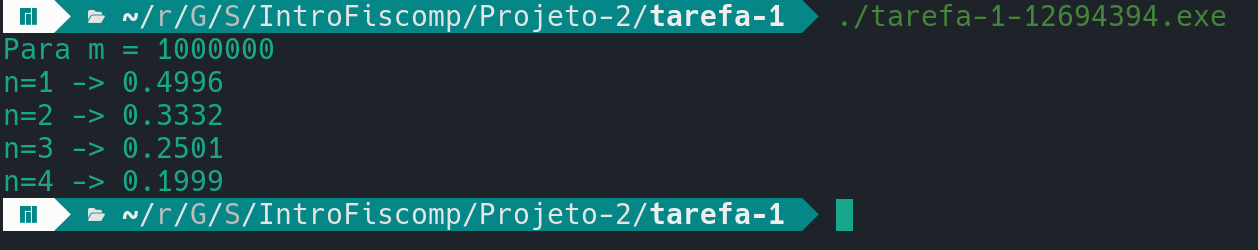
\includegraphics[width=14cm]{images/tarefa-1/imag1.png}
\caption*{Fonte: Compilado pelo Autor.}
\label{fig:tarefa 1 - código exibido na tela}
\end{figure}

\vspace*{2\baselineskip}

\begin{figure}[h!]
\centering
\caption{Valores de $\langle x^n \rangle$ para n entre 1 e 10}
  \centering
  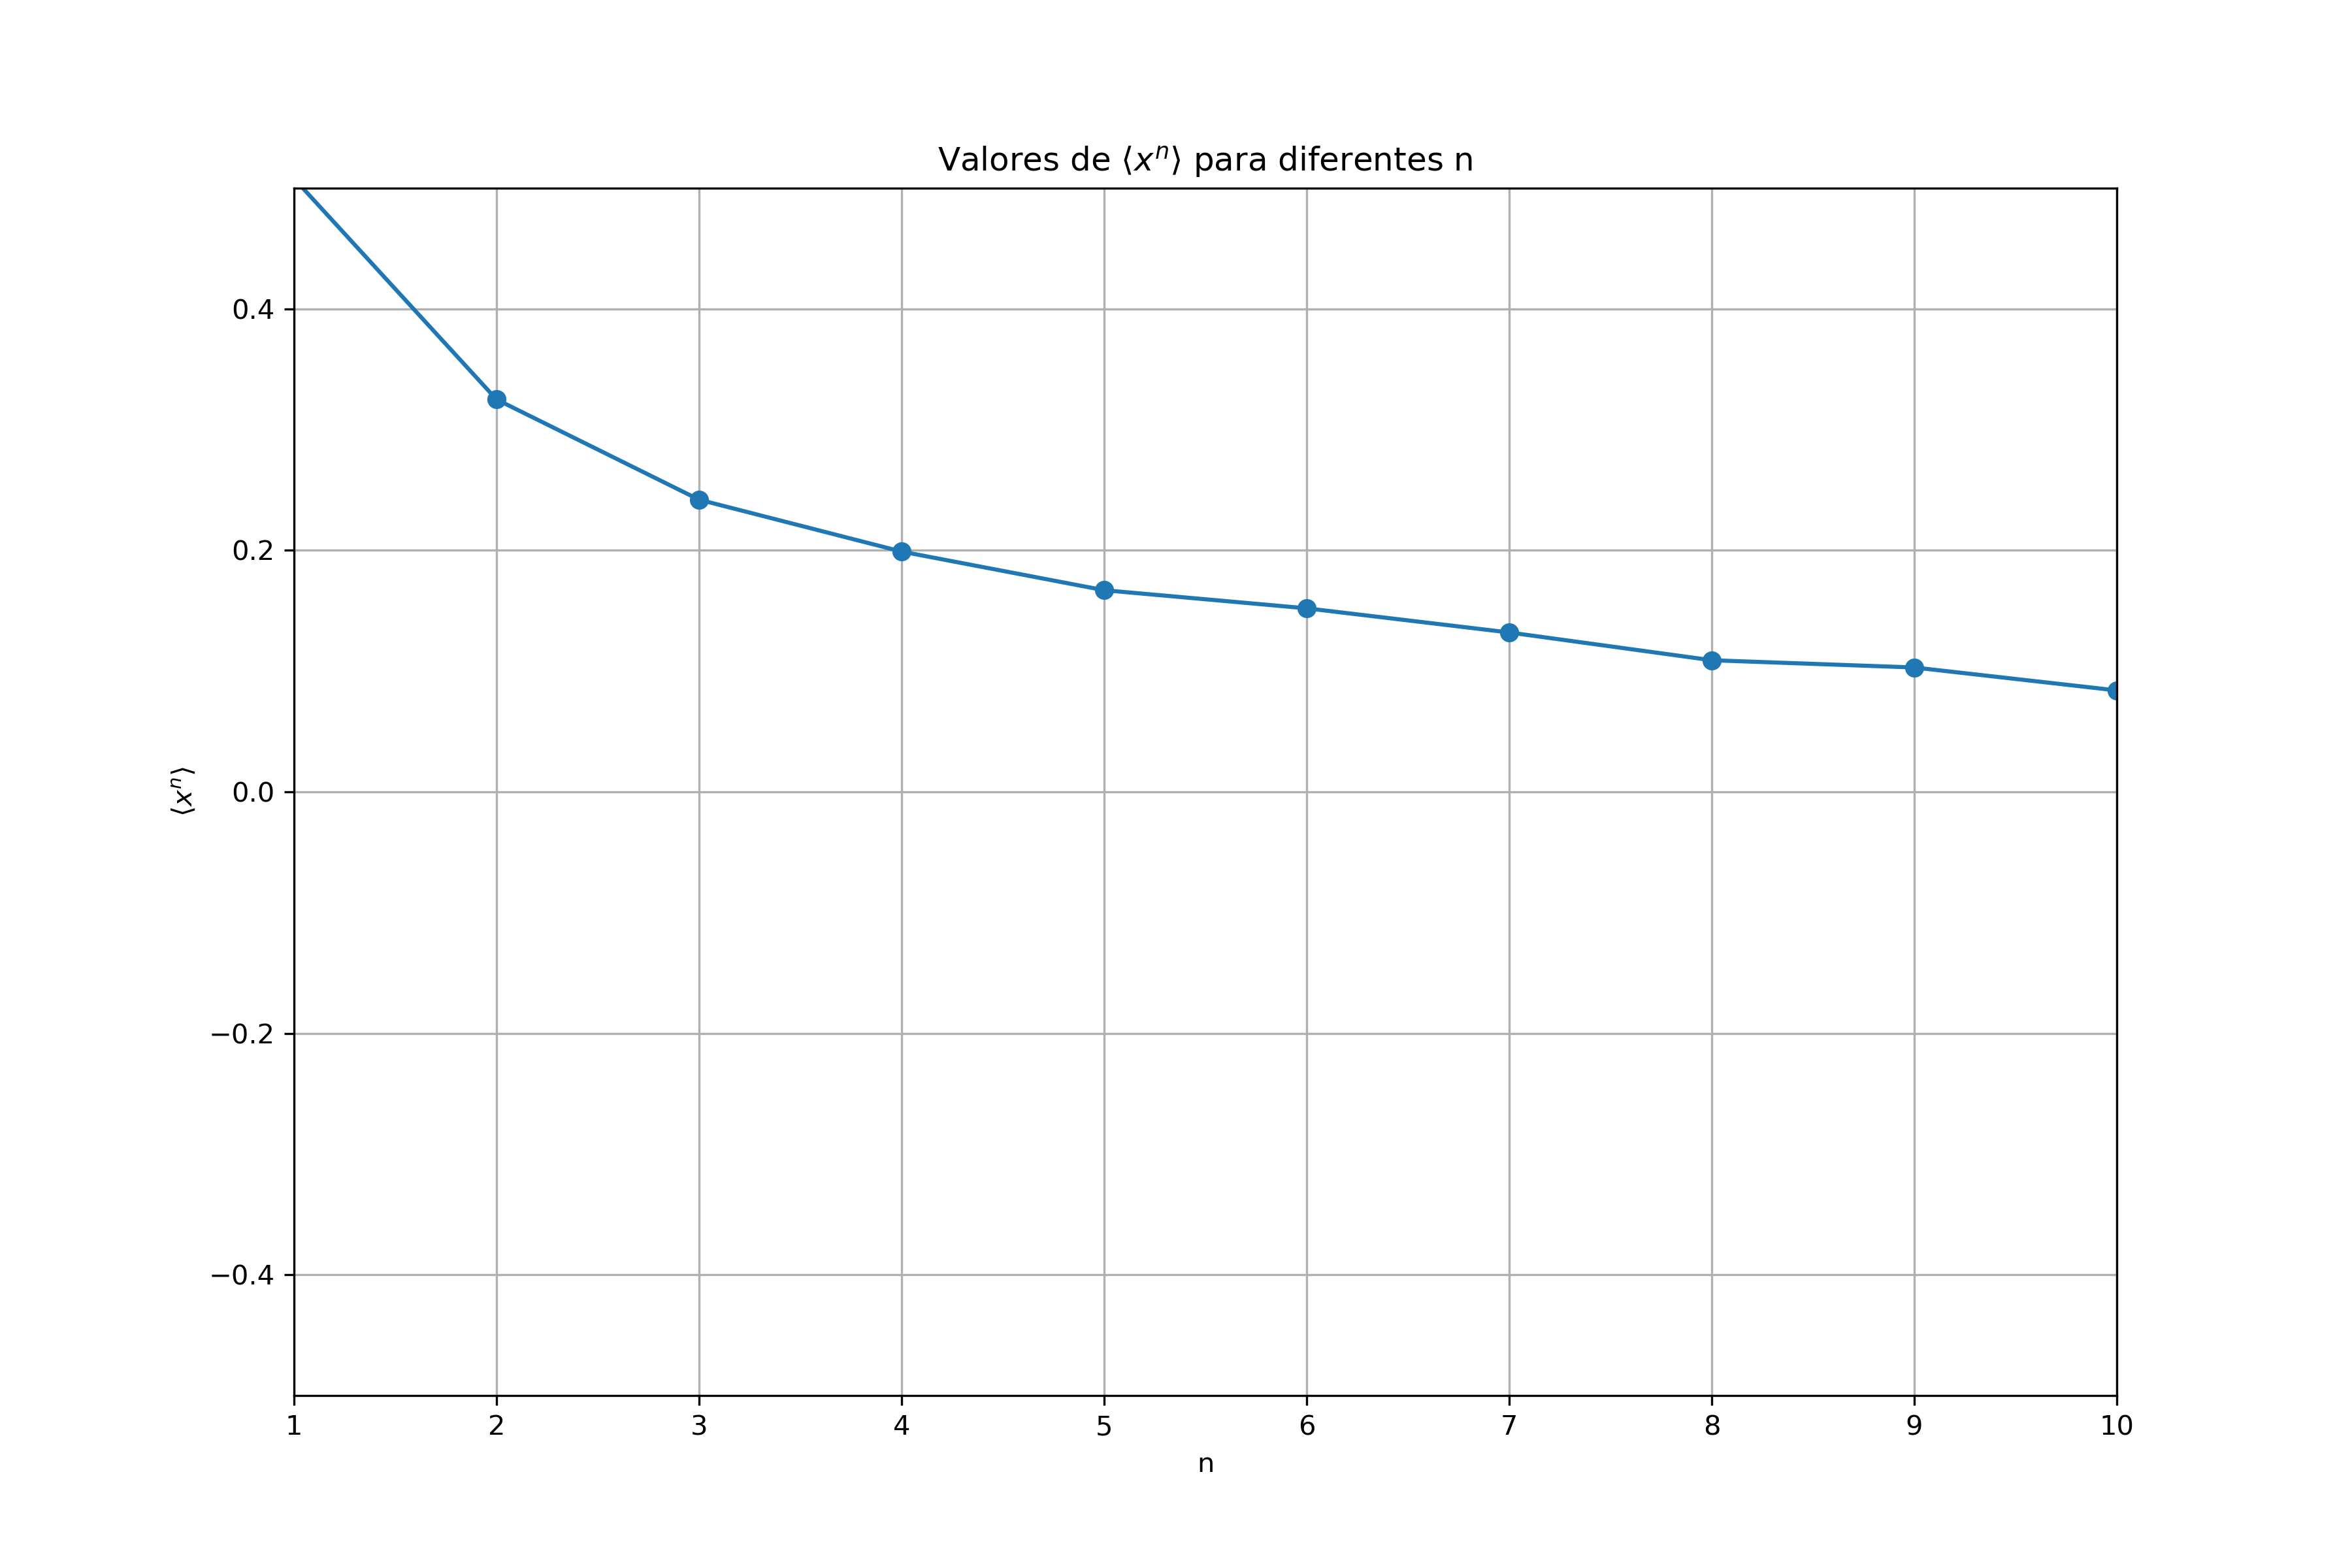
\includegraphics[width=14cm]{images/tarefa-1/fig_tarefa1_2.png}
\caption*{Fonte: Compilado pelo Autor.}
\label{fig:tarefa 1 - <x^n> para difererentes n =1,10}
\end{figure}

\vspace*{2\baselineskip}

\begin{figure}[h!]
\centering
\caption{Histograma que mostra a distribuição de valores para a função \textbf{rand()}, variando entre 0 e 1.}
  \centering
  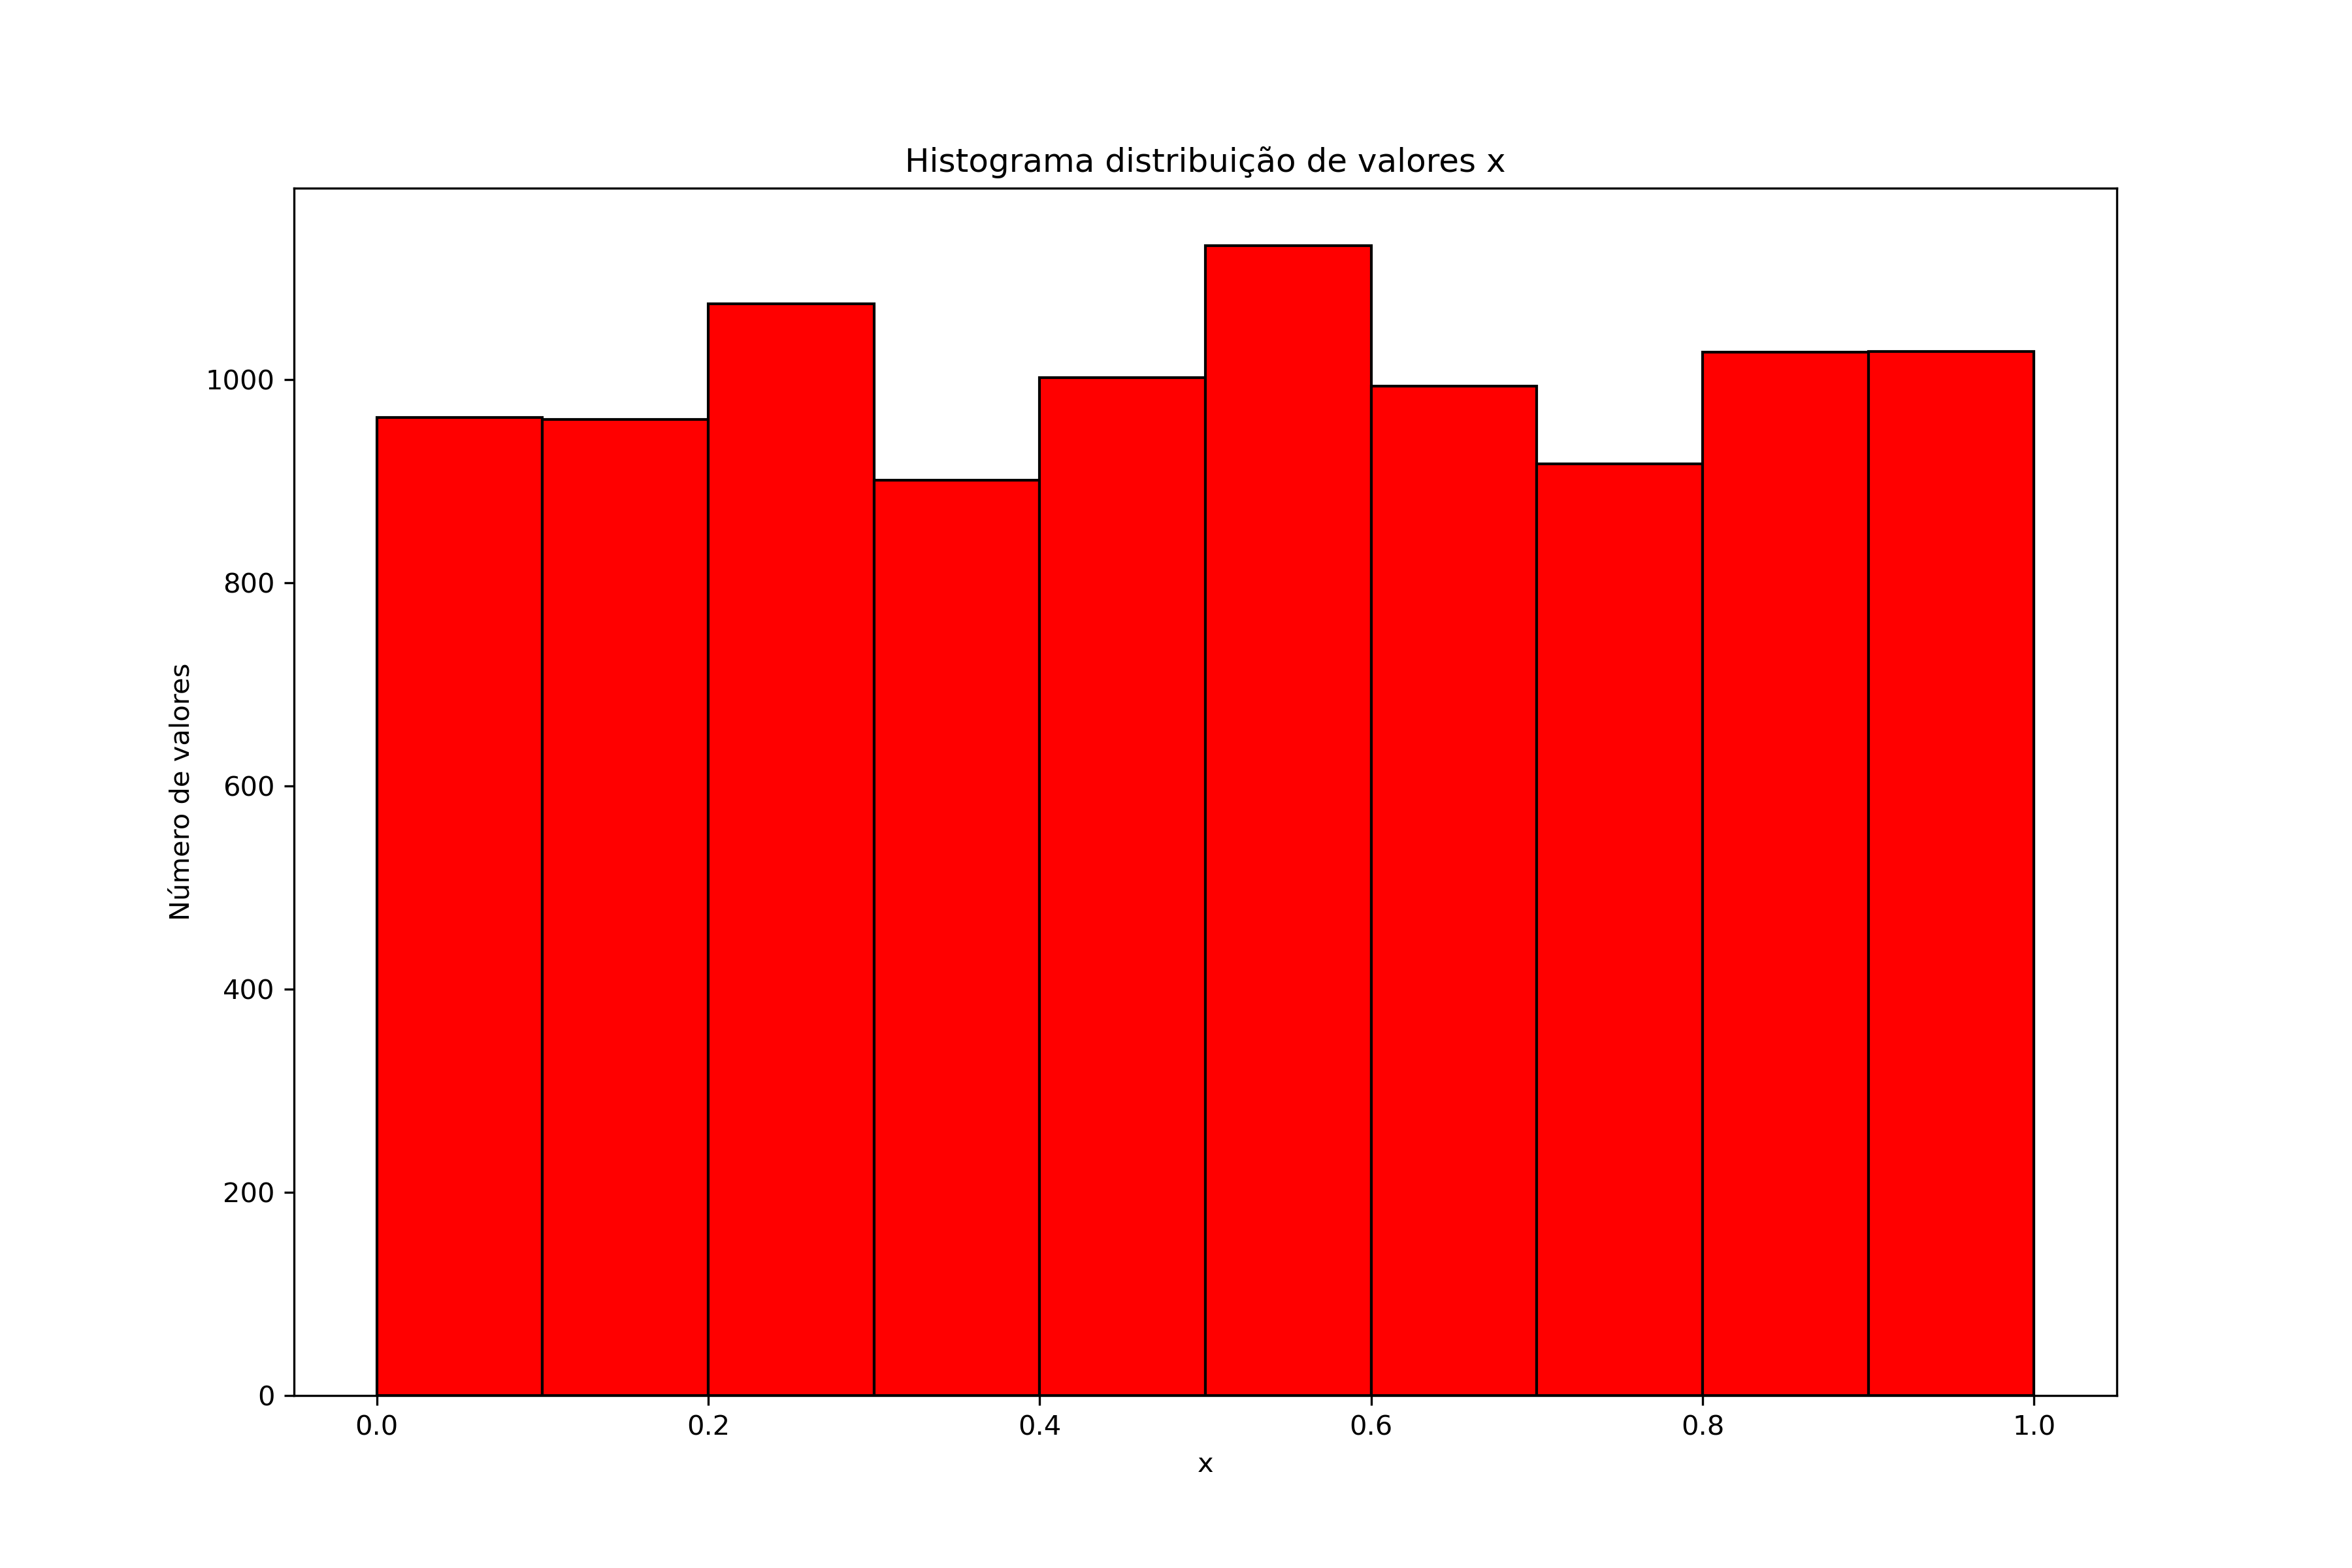
\includegraphics[width=14cm]{images/tarefa-1/fig_tarefa1_3.png}
\caption*{Fonte: Compilado pelo Autor.}
\label{fig:tarefa 1 - histograma rand()}
\end{figure}
